%% -*- TeX-engine: luatex; ispell-dictionary: "english" -*-

\documentclass[unicode,11pt]{beamer}

\PassOptionsToPackage{obeyspaces}{url}

\usetheme{Pittsburgh}
\usecolortheme{beaver}

\newenvironment{stopperenv}{\only{\setbeamercolor{local structure}{fg=darkred}}}{}

\setbeamercolor{frametitle}{fg=black,bg=white}
\setbeamerfont{frametitle}{size=\Large}
\setbeamertemplate{footline}[frame number]
\setbeamertemplate{frametitle continuation}{(\insertcontinuationcount)}
\setbeamertemplate{caption}{\insertcaption}
\setbeamertemplate{enumerate items}[default]
\setbeamertemplate{frametitle}{\hfill\insertframetitle\vskip-6pt\hrulefill}

\setbeamercovered{dynamic} % overlays not yet revealed will faintly appear
\beamertemplatenavigationsymbolsempty

\usepackage{fontspec}
\setmainfont{PT Serif}
\setsansfont{PT Sans}
\setmonofont[Ligatures=NoCommon]{PT Mono}
\defaultfontfeatures{Ligatures=TeX}

% sans serif for headings
\setbeamerfont*{block title}{family=\sffamily,series=\bfseries}

%\usepackage{microtype}


\newcommand{\theme}[1]{%
  \centering\fontsize{36pt}{1em}\color{darkred}{\selectfont{#1}}
}

\usepackage{polyglossia}
\setdefaultlanguage{english}
\usepackage{csquotes}

\usepackage[normalem]{ulem}

\usepackage{hyperref}
\hypersetup{
	colorlinks=true,
    linkcolor=darkred,
    urlcolor=darkred,
    citecolor=darkred
}

\makeatletter
\let\@mycite\@cite
\def\@cite#1#2{{\hypersetup{linkcolor=darkred}[{#1\if@tempswa , #2\fi}]}}
\makeatother

\usepackage{caption}
\captionsetup[figure]{labelformat=empty}

\usepackage{amsmath}
\usepackage{amssymb}
\DeclareMathOperator*{\argmin}{arg\,min}
\DeclareMathOperator*{\argmax}{arg\,max}

\newcommand{\op}[1]{\operatorname{#1}}


\usepackage{subcaption}
\usepackage{mathtools}  %% for \underbrace


\title{\large{Variational Auto-Encoder. Normalizing flows}}

\begin{document}

\begin{frame}[plain,noframenumbering]
  \maketitle
\end{frame}

\begin{frame}[fragile]{Latent variable generative models}
\textcolor{darkred}{Idea}: Learn a mapping from some latent variable $z$
to a complicated distribution on $x$.

$$p(x) = \int{p(x, z) dz} \qquad\text{where}\qquad p(x, z) = p(x|z)p(z)$$
$$p(z) = \text{something simple}  \qquad  p(x|z) = g(z)$$
\end{frame}


\begin{frame}[fragile]{Bayesian inference}
todo
\end{frame}


\begin{frame}[fragile]{Practical notes}
  \begin{itemize}
    \item Intractability
    \item Large dataset
  \end{itemize}
\end{frame}

\begin{frame}[fragile]{Solutions}
todo
\end{frame}

\begin{frame}[fragile]{Solution problems}
todo
\end{frame}

\begin{frame}[fragile]{Variational inference}
  \begin{itemize}
    \item Stochastic optimization
    \item Convergence
  \end{itemize}
\end{frame}


\begin{frame}[fragile]{Variational lower bound}
\begin{align*} 
\log {p_\theta (x)} &= \log \int {p_\theta (x|z) p(z) dz} \\
&= \log \int{ \frac{q_\phi (z|x)}{q_\phi (z|x)} p_\theta (x|z) p(z) dz} \\
&= -\mathbb{D}_{KL}[q_\phi (z|x) \parallel p(z)] + \mathbb{E}_q [\log p_\theta (x|z)]
\end{align*} 

\end{frame}

\begin{frame}[fragile]{Variational Auto-Encoder}
todo
\end{frame}

\begin{frame}[fragile]{VAE inference model}
\textcolor{darkred}{The VAE approach}: introduce an inference model that
learns to approximate the intractable posterior by
optimizing the variational lower bound: 
$$ \mathcal{L}(\theta, \phi, x) = -\mathbb{D}_{KL}[q_\phi (z|x) \parallel p(z)] + \mathbb{E}_q [\log p_\theta (x|z)] $$
We parameterize with another neural network:
\begin{figure}[htbp]
  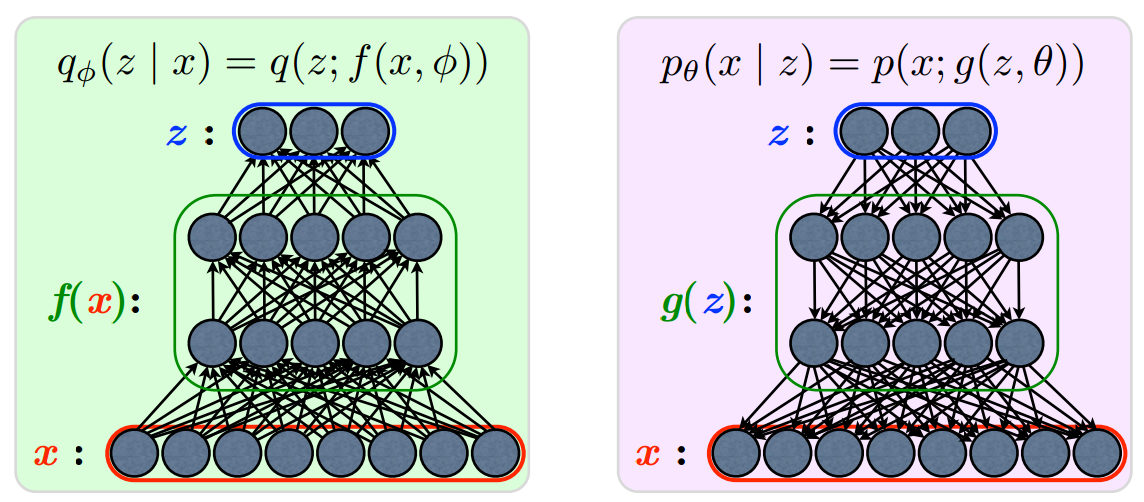
\includegraphics[height=130pt, keepaspectratio = true]{images/vae}   
\end{figure}

\end{frame}

\begin{frame}[fragile]{Reparametrization trick}
\begin{itemize}
  \item $q_\phi(z|x) = \mathcal{N}(z; \mu_z(x), \sigma_z(x))$
  \item Parametrize $z$ as $z = \mu_z(x) + \sigma_z(x)\varepsilon_z$ where $\varepsilon_z = \mathcal{N}(0, 1)$ 
\end{itemize}
\end{frame}

\begin{frame}[fragile]{Coding theory perspective}
The unobserved variables $z$ have an interpretation as a latent representation or code.

\begin{itemize}
  \item Represent recognition model $q_phi(z|x)$ as a probabilistic encoder.\\
        Given a datapoint $x$ it produces a distribution over the possible values of the code $z$ from which the datapoint $x$ could have been generated
  \item Represent $p\theta(x|z)$ as a probabilistic decoder.\\
        Given a code $z$ it produces a distribution over the possible corresponding values of $x$
\end{itemize}
\end{frame}

\begin{frame}[fragile]{Model restriction}
Diagonal covariance\\
\vspace{5mm}
What can be done?
\end{frame}


\begin{frame}[fragile]{Normalizing flows}
\textcolor{darkred}{Normalizing flows}: the transformation of a probability density through
a sequence of invertible mappings.
\begin{itemize}
  \item By repeated application of the rule for random variable transformations, the initial
density flows through the sequence of invertible mappings.
  \item At the end of the sequence, we have a valid probability distribution.
\end{itemize}

\end{frame}

\begin{frame}[fragile]{Normalizing flows}
Transformation of random variables: $z' = f(z)$, $f^{-1}(z') = z$\\
$$q(z') = q(z) \left\vert \det \frac{\partial f^{-1}(z')}{\partial z'} \right\vert = 
q(z) \left\vert \det \frac{\partial f(z')}{\partial z'} \right\vert^{-1}$$\\
Chaining together a sequence: $z_K = f_K \circ f_{K−1} \circ \cdots \circ f_2 \circ f_1(z_0)$\\
$$\log q_K(z_K) = \log q_0(z_0) − \sum_{k=1}^K \log \left\vert \det \frac{\partial f_k}{\partial z_k} \right\vert $$

Law of the unconscious statistician:\\
$$\mathbb{E}_{q_K} \left[g(z_K)\right] = \mathbb{E}_{q_0} \left[ g(f_K \circ f_{K−1} \circ \cdots \circ f_2 \circ f_1(z_0)) \right] $$
\end{frame}

\begin{frame}[fragile]{Variational lower bound}
\begin{align*} 
\mathcal{L}(\theta, \phi, x) &= \mathbb{E}_{q_\phi(z|x)} \left[ \log p_\theta(x, z) - \log q_\phi(z | x) \right] \\
&= \mathbb{E}_{q_K(z_K)} \left[ \log p(x, z_K) - \log q(z_K) \right] \\
&= \mathbb{E}_{q_0(z_0)} \left[ \log p(x, z_K) - \log q0(z_0) + \sum_{k=1}^K \log \left\vert \det \frac{\partial f_k}{\partial z_k} \right\vert \right] 
\end{align*} 
\end{frame}

\begin{frame}[fragile]{Planar flow}
Family of transformations: $f(z) = z + uh(w^⊤z + b)$\\
\vspace{5mm}
$$\left\vert \det \frac{\partial f(z)}{\partial z} \right\vert = \left\vert 1 + u^T \psi(z) \right\vert \text{where} \psi(z) = h'(w^⊤z + b)w$$ \\
$$\log q_K(z_K) = \log q_0(z_0) − \sum_{k=1}^K \log \left\vert 1 + u^T \psi(z) \right\vert $$
\end{frame}

\begin{frame}[fragile]{Radial flow}
todo
\end{frame}


\begin{frame}[fragile]{Results}
todo
\end{frame}

\begin{frame}[fragile]{Future experiments}
todo 
\end{frame}

\end{document}
